\documentclass[10 pt,usenames,dvipsnames, oneside]{article}
\usepackage{../../../modelo-ensino-medio}



\begin{document}

\begin{center}
  \begin{minipage}[l]{3cm}

\includegraphics[width=2cm]{logo}    
\end{minipage}\hfill
\begin{minipage}[r]{.8\textwidth}
 {\Large \scshape Atividade: Expoentes racionais}  
\end{minipage}
\end{center}
\vspace{.2cm}

\ifdefined\prof
%Habilidades da BNCC
\begin{objetivos}
\item \textbf{EM13MAT403} Comparar e analisar as representações, em plano cartesiano, das funções exponencial e logarítmica para identificar as características fundamentais (domínio, imagem, crescimento) de cada uma, com ou sem apoio de tecnologias digitais, estabelecendo relações entre elas.
\end{objetivos}

%Caixa do Para o Professor
\begin{goals}
%Objetivos específicos
\begin{enumerate}
\item Revisar as propriedades aritméticas das potências com expoentes racionais;
\item Construir de modo intuitivo o significado de potências com expoentes inteiros racionais;
\end{enumerate}

\tcblower

%Orientações e sugestões
\begin{itemize}
\item Esta atividade guarda bastantes semelhanças com a anterior, no sentido de que pode ser feita de maneira investigativa e que se trata de uma ampliação da definição de potência para expoentes racionais;

\item Alguns estudantes podem optar por representar os racionais na forma decimal e isto pode dificultar a percepção dos padrões. Sugira que estes também considerem trabalhar com frações;

\item Para muitos estudantes esse tema já deve ser conhecido do Ensino Fundamental, mas acreditamos que a maneira como expomos pode ajudar a construir uma intuição das justificativas/demonstrações das propriedades com expoentes racionais;

\item Essa intuição servirá de base para as discussões envolvendo a função exponencial de domínio real, onde abordaremos o cálculo do fator de crescimento, ou a imagem da função exponencial para tempos não inteiros.
\end{itemize}
\end{goals}

\bigskip
\begin{center}
{\large \scshape Atividade}
\end{center}
\fi

Observe os cartões e responda as perguntas.

\begin{enumerate}

\item{}
Completes os cartões vazios nas sequências abaixo. Explique seu raciocínio.

\begin{figure}[H]
\centering
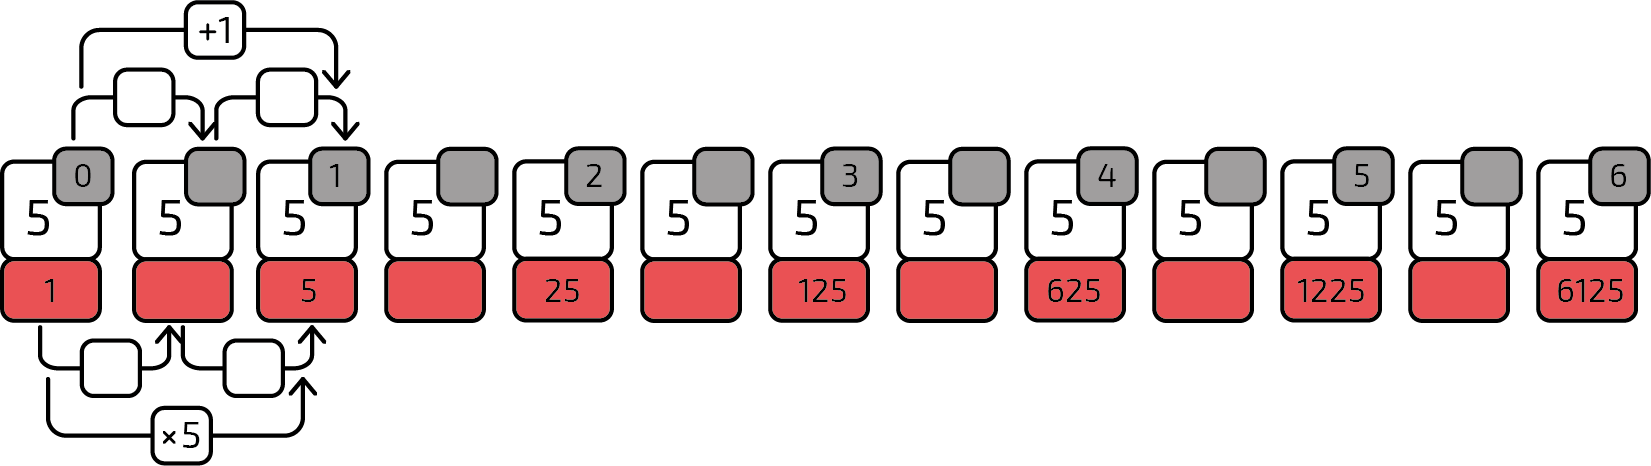
\includegraphics[width=350bp]{aritm11.png}
\end{figure}


\begin{figure}[H]
\centering
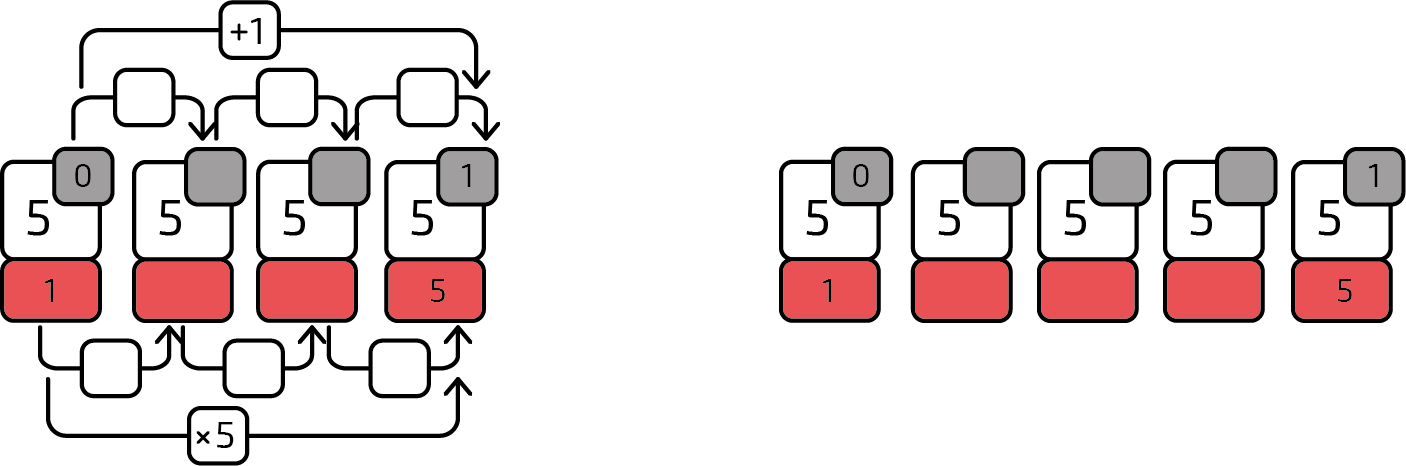
\includegraphics[width=300bp]{aritm12.png}
\end{figure}

\item{}
Represente nos cartões abaixo as expressões pedidas:

\begin{figure}[H]
\centering
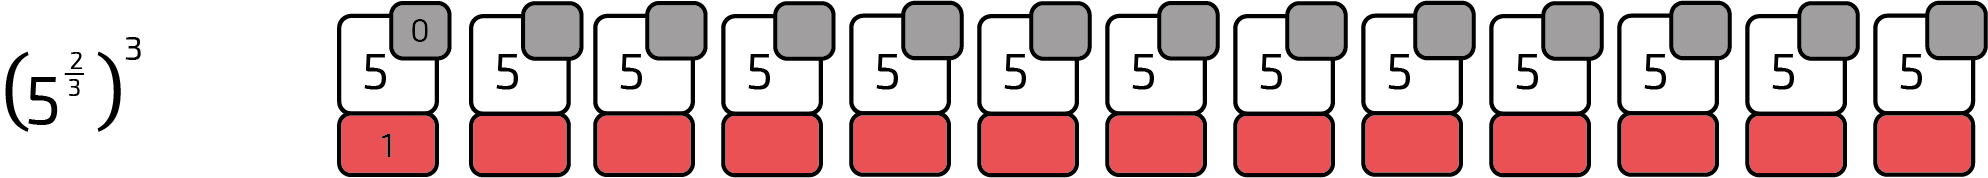
\includegraphics[width=350bp]{aritm13.png}
\end{figure}

\begin{figure}[H]
\centering
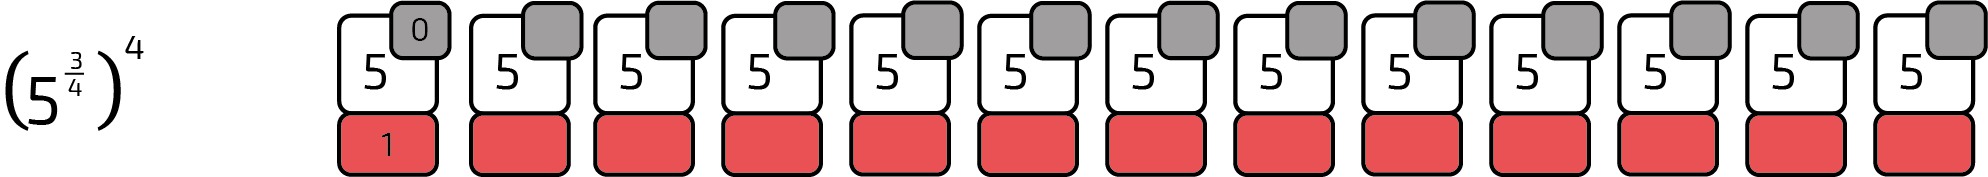
\includegraphics[width=350bp]{aritm14.png}
\end{figure}

\begin{figure}[H]
\centering
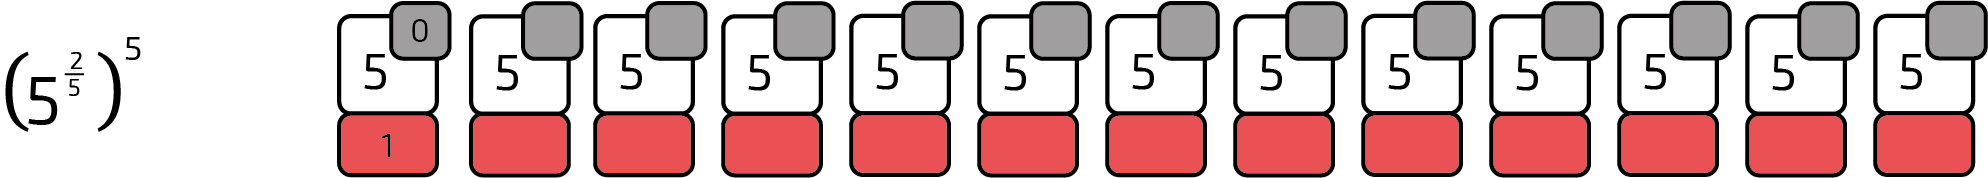
\includegraphics[width=350bp]{aritm15.png}
\end{figure}

\item{}
Qual a sua conclusão sobre que significado tem a expressão $5^{\frac{m}{n}}$ ?

\end{enumerate}

\ifdefined\prof
\begin{solucao}

\begin{enumerate}
\item Completando os cartões obtemos:

\begin{figure}[H]
\centering
\noindent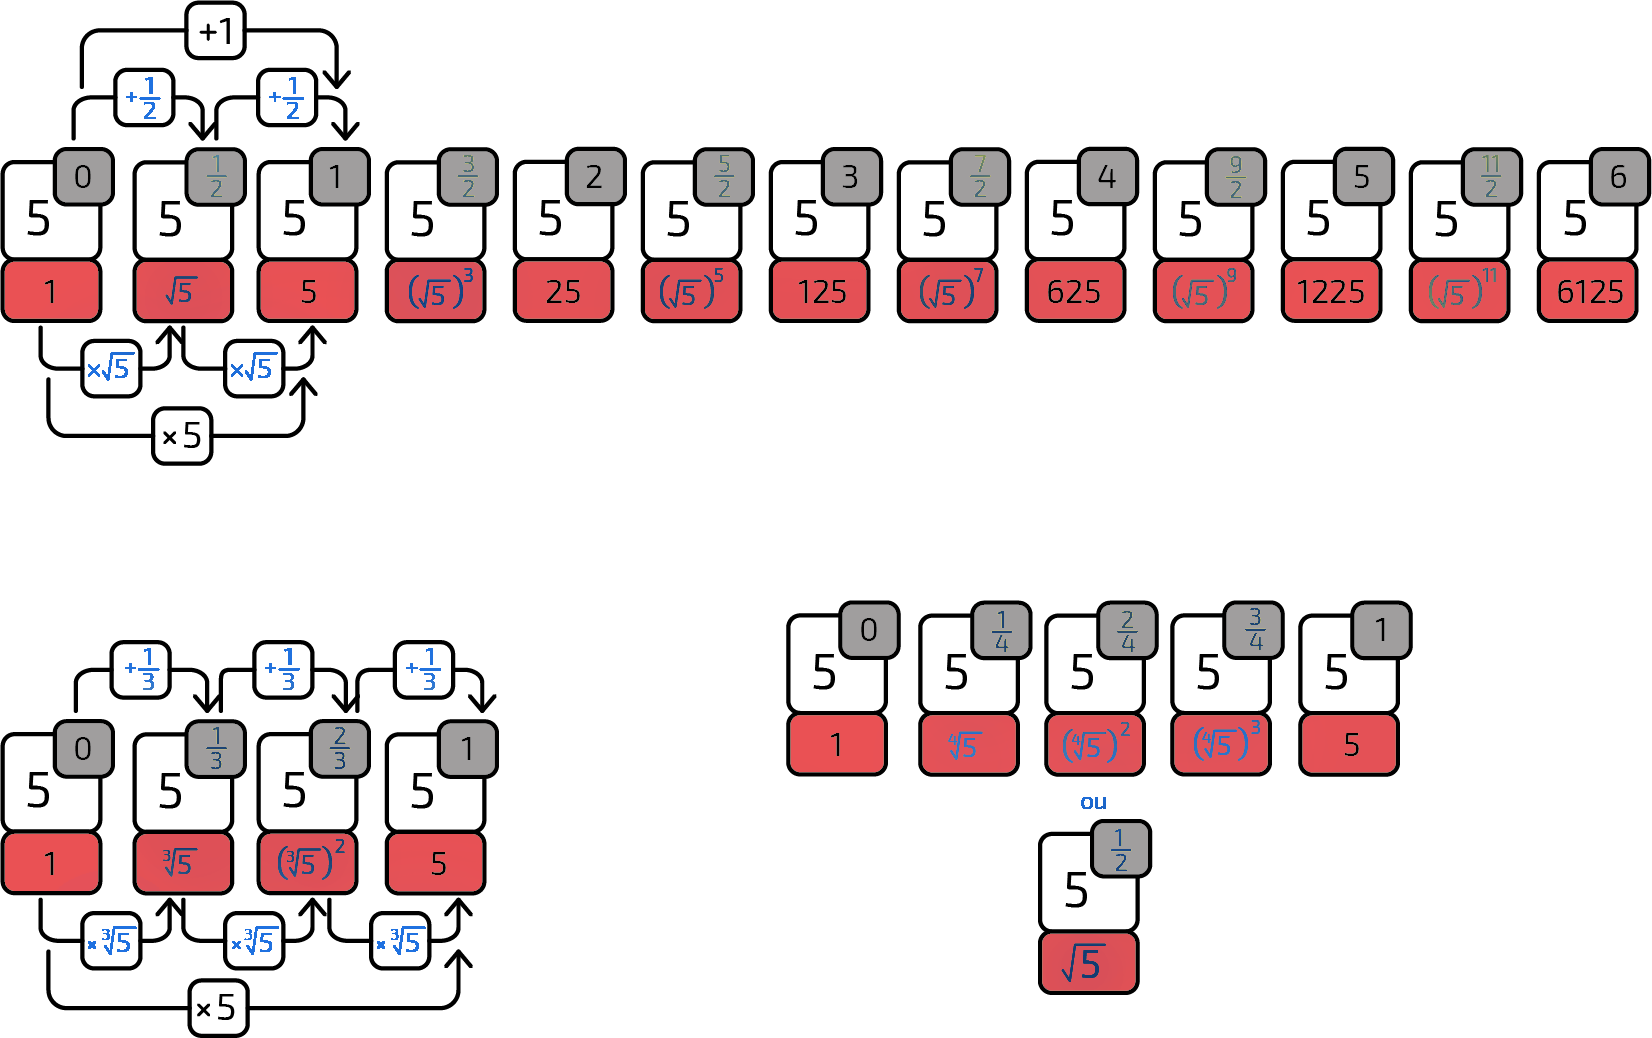
\includegraphics[width=.75\linewidth]{resp_racionais_a.png}
\end{figure}

\item As expressões serão representadas por:

\begin{figure}[H]
\centering
\noindent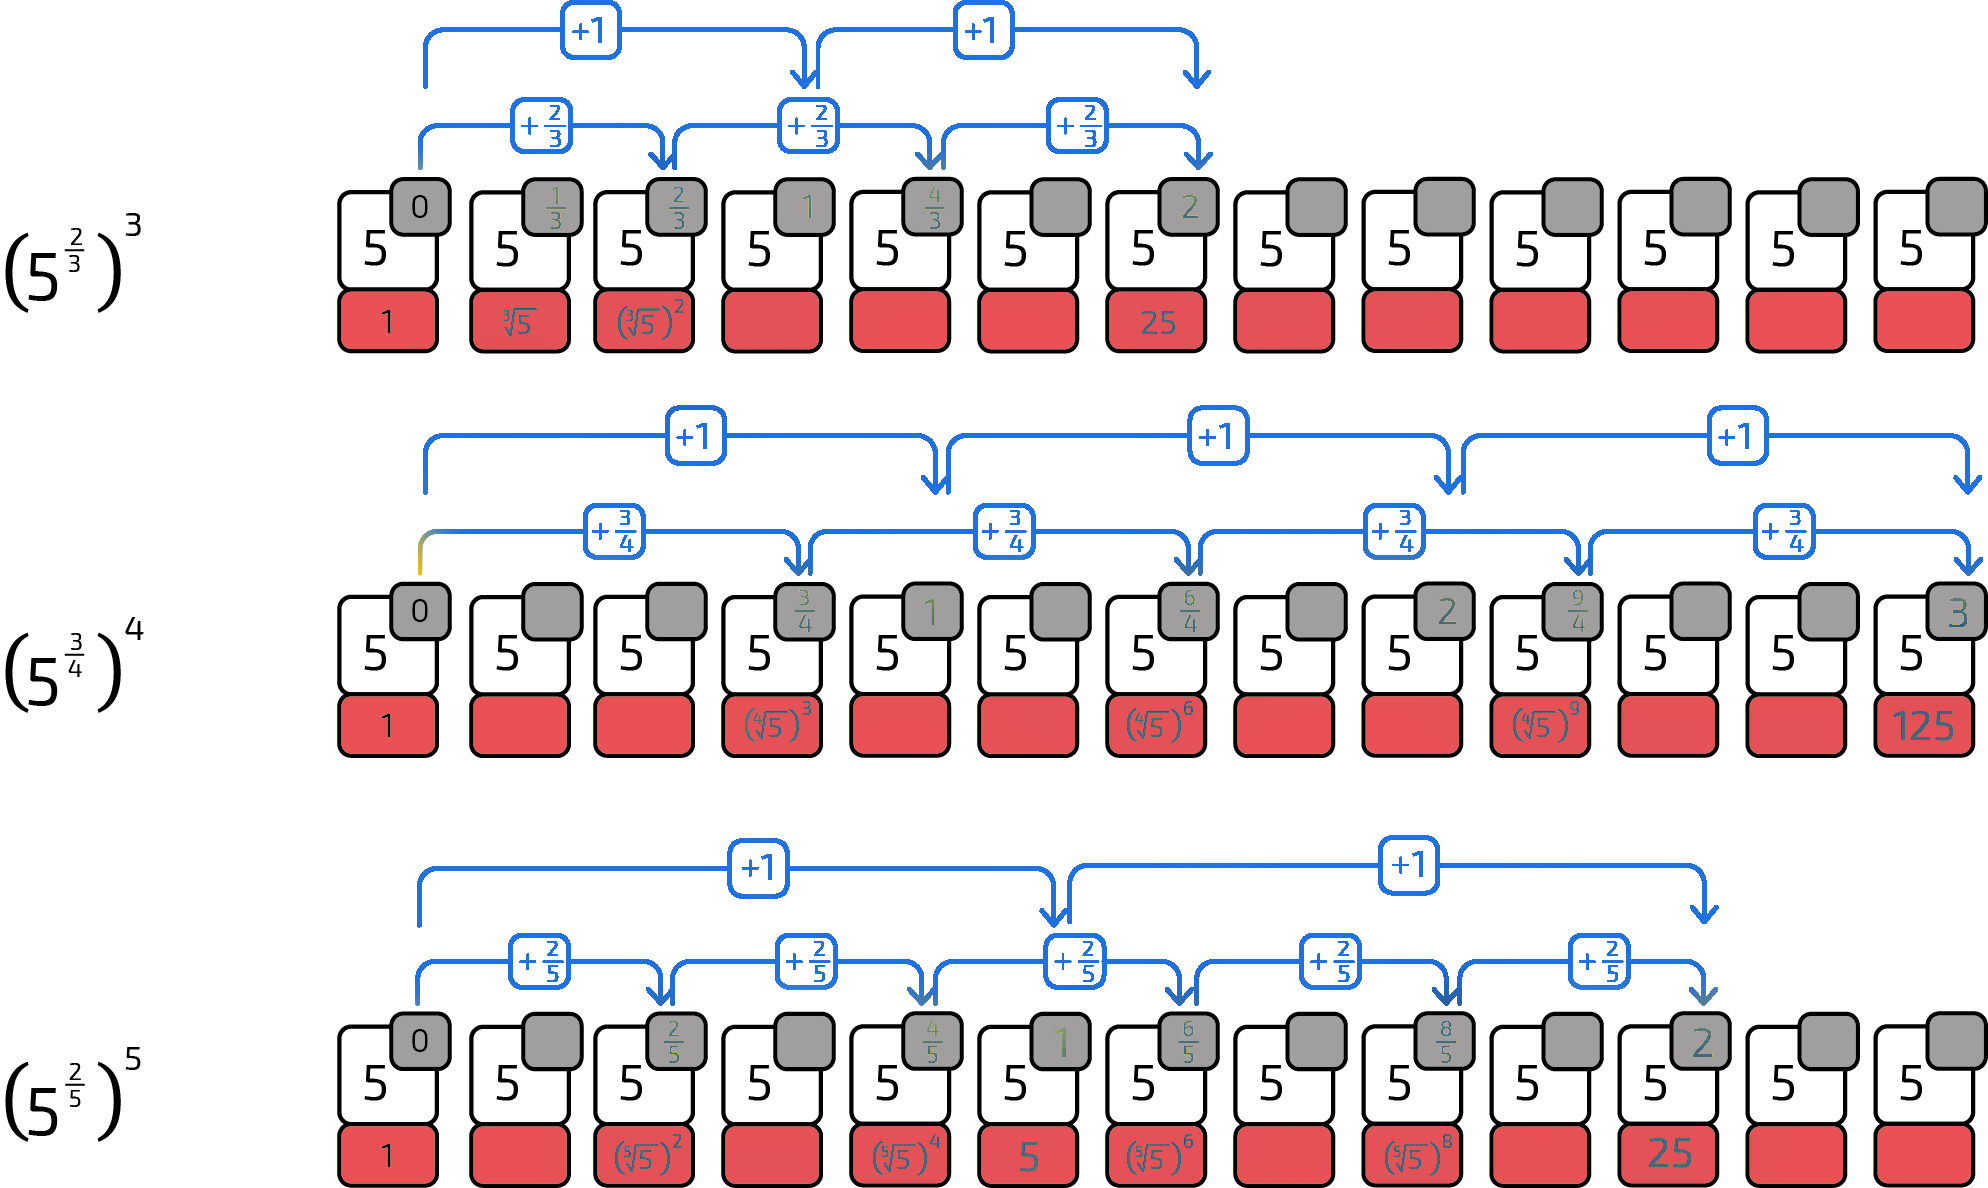
\includegraphics[width=.75\linewidth]{resp_racionais_b.png}
\end{figure}

\item $5^{\frac{m}{n}}=(\sqrt[n]{5})^{m}$.

\end{enumerate}

\end{solucao}
\fi

\end{document}